% questions.tex —— 2011 年·四川卷·文科 · 题目内容片段（无答案）
% 由 tools/generate_projects.py 依来源总账自 2011/2011_数学真题_四川文_试题.md 生成，勿手改（改源 MD 后重跑）


\gkpart{数学}

\begin{gktip}
\textbf{来源说明}：本题面依据固定源 PDF 两页 A3 题面逐栏转录，原卷印刷页码 703–704。固定源不附答案；原页各题与各节均未印分值，记「原页未标」，不补。答案和解析均由本库独立复算。

\textbf{源疑点}：第 7 题（A）选项在原页印作粗体「0」，按零向量 $\boldsymbol 0$ 转录。第 20 题第（1）问中，若把 $q=0$ 也当作公比代入，$2S_3=S_1+S_4$ 亦成立，但等比数列的定义要求公比 $q\neq0$（$q=0$ 时从第三项起出现 $0/0$，不满足「每项与前一项之比为同一常数」），本库按 $q\neq0$ 取解，题面照录；详见解析正文。

\textbf{图形说明}：第 4 题四个选项的函数图象、第 7 题的正六边形、第 15 题的球与内接圆柱、第 19 题的直三棱柱、第 21 题的椭圆与直线 $l$ 均重绘为 TikZ 矢量图，依原页拓扑重绘，不按比例。原页其余各题无图。
\end{gktip}

\gkpart{一、选择题}

\begin{question}
\gkti{1}若全集 $M=\{1,2,3,4,5\}$，$N=\{2,4\}$，则 $\complement_M N=$\mbox{（　　）}

（A）$\varnothing$

（B）$\{1,3,5\}$

（C）$\{2,4\}$

（D）$\{1,2,3,4,5\}$

\end{question}
\begin{question}
\gkti{2}有一容量为 $66$ 的样本，数据的分组及各组的频数如下：

\nopagebreak[4]
\[[11.5,15.5)\ \ 2 \qquad [15.5,19.5)\ \ 4 \qquad [19.5,23.5)\ \ 9 \qquad [23.5,27.5)\ \ 18\]

\nopagebreak[4]
\[[27.5,31.5)\ \ 11 \qquad [31.5,35.5)\ \ 12 \qquad [35.5,39.5)\ \ 7 \qquad [39.5,43.5)\ \ 3\]

根据样本的频率分布估计，大于或等于 $31.5$ 的数据约占\mbox{（　　）}

（A）$\dfrac{2}{11}$

（B）$\dfrac13$

（C）$\dfrac12$

（D）$\dfrac23$

\end{question}
\begin{question}
\gkti{3}圆 $x^2+y^2-4x+6y=0$ 的圆心坐标是\mbox{（　　）}

（A）$(2,3)$

（B）$(-2,3)$

（C）$(-2,-3)$

（D）$(2,-3)$

\Needspace{0.4\textheight}
\end{question}
\begin{question}
\gkti{4}函数 $y=\left(\dfrac12\right)^x+1$ 的图象关于直线 $y=x$ 对称的图象大致是\mbox{（　　）}

（A）图 A

（B）图 B

（C）图 C

（D）图 D
\nopagebreak[4]
\begin{center}% 2011 年四川卷文科第 4 题：四个选项的函数图象（选项图）。
% 来源 PDF：普通高考/2011/2011四川文.pdf，SHA-256 9df4a6b69bb06bfab2f7d7ee0e7fcc50ae547f226260996d7a060c31ad14e64a。
% 原页：第 1 页（A3 三栏）第 1 栏中部，书页码 703。
% 重绘依据：照原页——(A) 递减、竖直渐近线 x=1、过 (2,0)，y 轴标 1、x 轴标 1 与 2；
%   (B) 递增、竖直渐近线 x=1、过 (2,0)，y 轴标 1、x 轴标 1 与 2；
%   (C) 递增、过 (0,2)、水平渐近线 y=1，y 轴标 2（曲线与 y 轴交点处）与 1，x 轴标 1；
%   (D) 递增、与 x 轴交点处标 −2、x 轴另标 −1、y 轴标 1，左端渐平（渐近线在 x 轴下方）。
%   四个选项各为独立的直角坐标系，(A)(B) 在上行、(C)(D) 在下行，字母在各自图形左下，照原页。
%   说明：(D) 只是干扰项，原页未给函数式，仅按可辨认的拓扑（增、下凸、在负半轴穿过 x 轴、
%   y 轴截距 1、左端有水平渐近线）重绘，取 y=2^{x/2+1}-1 作图，不按原页比例，不代表某个确定函数。
%   原页各图均无网格、无虚线。
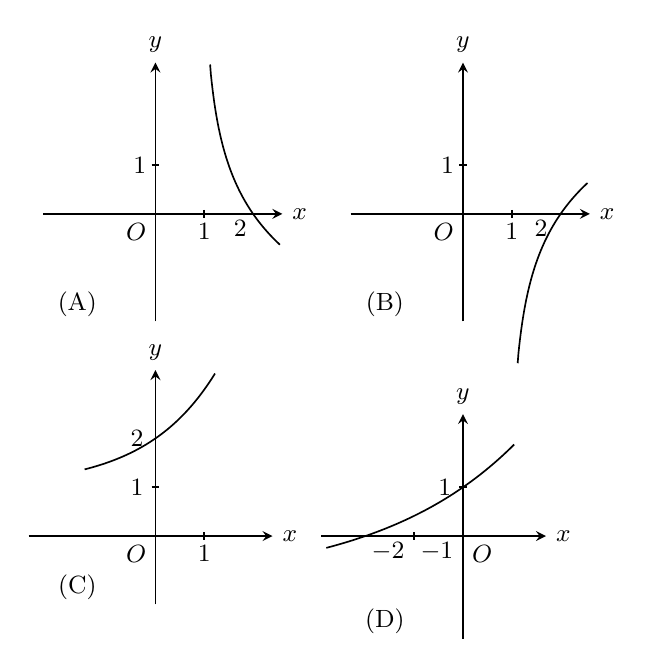
\begin{tikzpicture}[scale=0.62, >=stealth, semithick, font=\small]

  % ================= (A) =================
  \begin{scope}
    \draw[->] (-2.3,0) -- (2.6,0) node[right] {$x$};
    \draw[->] (0,-2.2) -- (0,3.1) node[above] {$y$};
    \draw (1,0.08) -- (1,-0.08);
    \draw (-0.08,1) -- (0.08,1);
    \node[below left, inner sep=3pt] at (0,0) {$O$};
    \node[below, inner sep=3pt] at (1,0) {$1$};
    \node[below left, inner sep=2pt] at (2,0) {$2$};
    \node[left, inner sep=3pt] at (0,1) {$1$};
    \draw[domain=1.12:2.55, samples=90] plot (\x,{-ln(\x-1)/ln(2)});
    \node at (-1.6,-1.85) {(A)};
  \end{scope}

  % ================= (B) =================
  \begin{scope}[shift={(6.3,0)}]
    \draw[->] (-2.3,0) -- (2.6,0) node[right] {$x$};
    \draw[->] (0,-2.2) -- (0,3.1) node[above] {$y$};
    \draw (1,0.08) -- (1,-0.08);
    \draw (-0.08,1) -- (0.08,1);
    \node[below left, inner sep=3pt] at (0,0) {$O$};
    \node[below, inner sep=3pt] at (1,0) {$1$};
    \node at (1.60,-0.30) {$2$};
    \node[left, inner sep=3pt] at (0,1) {$1$};
    \draw[domain=1.12:2.55, samples=90] plot (\x,{ln(\x-1)/ln(2)});
    \node at (-1.6,-1.85) {(B)};
  \end{scope}

  % ================= (C) =================
  \begin{scope}[shift={(0,-6.6)}]
    \draw[->] (-2.6,0) -- (2.4,0) node[right] {$x$};
    \draw[->] (0,-1.4) -- (0,3.4) node[above] {$y$};
    \draw (1,0.08) -- (1,-0.08);
    \draw (-0.08,1) -- (0.08,1);
    \node[below left, inner sep=3pt] at (0,0) {$O$};
    \node[below, inner sep=3pt] at (1,0) {$1$};
    \node[left, inner sep=4pt] at (0,1) {$1$};
    \node[left, inner sep=4pt] at (0,2) {$2$};
    \draw[domain=-1.45:1.22, samples=90] plot (\x,{exp(\x*ln(2))+1});
    \node at (-1.6,-1.05) {(C)};
  \end{scope}

  % ================= (D) =================
  \begin{scope}[shift={(6.3,-6.6)}]
    \draw[->] (-2.9,0) -- (1.7,0) node[right] {$x$};
    \draw[->] (0,-2.1) -- (0,2.5) node[above] {$y$};
    \draw (-1,0.08) -- (-1,-0.08);
    \draw (-0.08,1) -- (0.08,1);
    \node[below right, inner sep=3pt] at (0,0) {$O$};
    \node[below right, inner sep=2pt] at (-2,0) {$-2$};
    \node[below right, inner sep=2pt] at (-1,0) {$-1$};
    \node[left, inner sep=4pt] at (0,1) {$1$};
    \draw[domain=-2.8:1.05, samples=90] plot (\x,{exp((\x/2+1)*ln(2))-1});
    \node at (-1.6,-1.75) {(D)};
  \end{scope}

\end{tikzpicture}
\end{center}
\nopagebreak[4]
\end{question}
\begin{question}
\gkti{5}“$x=3$”是“$x^2=9$”的\mbox{（　　）}

（A）充分而不必要的条件

（B）必要而不充分的条件

（C）充要条件

（D）既不充分也不必要的条件

\end{question}
\begin{question}
\gkti{6}$l_1$，$l_2$，$l_3$ 是空间三条不同的直线，则下列命题正确的是\mbox{（　　）}

（A）$l_1\perp l_2$，$l_2\perp l_3\Rightarrow l_1\parallel l_3$

（B）$l_1\perp l_2$，$l_2\parallel l_3\Rightarrow l_1\perp l_3$

（C）$l_1\parallel l_2\parallel l_3\Rightarrow l_1$，$l_2$，$l_3$ 共面

（D）$l_1$，$l_2$，$l_3$ 共点 $\Rightarrow l_1$，$l_2$，$l_3$ 共面

\Needspace{0.4\textheight}
\end{question}
\begin{question}
\gkti{7}如图，正六边形 $ABCDEF$ 中，$\overrightarrow{BA}+\overrightarrow{CD}+\overrightarrow{EF}=$\mbox{（　　）}

（A）$\boldsymbol 0$

（B）$\overrightarrow{BE}$

（C）$\overrightarrow{AD}$

（D）$\overrightarrow{CF}$
\nopagebreak[4]
\begin{center}% 2011 年四川卷文科第 7 题：正六边形 ABCDEF，求 \vec{BA}+\vec{CD}+\vec{EF}。
% 来源 PDF：普通高考/2011/2011四川文.pdf，SHA-256 9df4a6b69bb06bfab2f7d7ee0e7fcc50ae547f226260996d7a060c31ad14e64a。
% 原页：第 1 页（A3 三栏）第 1 栏下部，书页码 703。
% 重绘依据：照原页——上边 DE 水平、下边 BA 水平，D 在左上、E 在右上、C 在左、F 在右，
%   B 在左下、A 在右下；按正六边形作图，原页不画顶点圆点、不画对角线。
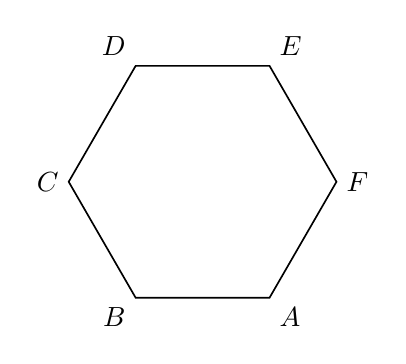
\begin{tikzpicture}[scale=1.7, >=stealth, semithick]
  \coordinate (A) at (0.5,-0.8660);
  \coordinate (B) at (-0.5,-0.8660);
  \coordinate (C) at (-1,0);
  \coordinate (D) at (-0.5,0.8660);
  \coordinate (E) at (0.5,0.8660);
  \coordinate (F) at (1,0);
  \draw (A) -- (B) -- (C) -- (D) -- (E) -- (F) -- cycle;
  \node at (A) [below right] {$A$};
  \node at (B) [below left] {$B$};
  \node at (C) [left] {$C$};
  \node at (D) [above left] {$D$};
  \node at (E) [above right] {$E$};
  \node at (F) [right] {$F$};
\end{tikzpicture}
\end{center}
\nopagebreak[4]
\end{question}
\begin{question}
\gkti{8}在 $\triangle ABC$ 中，$\sin^2A\leqslant\sin^2B+\sin^2C-\sin B\sin C$，则 $A$ 的取值范围是\mbox{（　　）}

（A）$\left(0,\dfrac{\pi}{6}\right]$

（B）$\left[\dfrac{\pi}{6},\pi\right)$

（C）$\left(0,\dfrac{\pi}{3}\right]$

（D）$\left[\dfrac{\pi}{3},\pi\right)$

\end{question}
\begin{question}
\gkti{9}数列 $\{a_n\}$ 的前 $n$ 项和为 $S_n$，若 $a_1=1$，$a_{n+1}=3S_n$（$n\geqslant1$），则 $a_6=$\mbox{（　　）}

（A）$3\times4^4$

（B）$3\times4^4+1$

（C）$4^5$

（D）$4^5+1$

\end{question}
\begin{question}
\gkti{10}某运输公司有 $12$ 名驾驶员和 $19$ 名工人，有 $8$ 辆载重量为 $10$ 吨的甲型卡车和 $7$ 辆载重量为 $6$ 吨的乙型卡车。某天需运往 $A$ 地至少 $72$ 吨的货物，派用的每辆车需载满且只运送一次，派用的每辆甲型卡车需配 $2$ 名工人，运送一次可得利润 $450$ 元；派用的每辆乙型卡车需配 $1$ 名工人，运送一次可得利润 $350$ 元。该公司合理计划当天派用甲、乙卡车的车辆数，可得最大利润 $z=$\mbox{（　　）}

（A）$4650$ 元

（B）$4700$ 元

（C）$4900$ 元

（D）$5000$ 元

\end{question}
\begin{question}
\gkti{11}在抛物线 $y=x^2+ax-5$（$a\neq0$）上取横坐标为 $x_1=-4$，$x_2=2$ 的两点，经过两点引一条割线，有平行于该割线的一条直线同时与抛物线和圆 $5x^2+5y^2=36$ 相切，则抛物线顶点的坐标为\mbox{（　　）}

（A）$(-2,-9)$

（B）$(0,-5)$

（C）$(2,-9)$

（D）$(1,-6)$

\end{question}
\begin{question}
\gkti{12}在集合 $\{1,2,3,4,5\}$ 中任取一个偶数 $a$ 和一个奇数 $b$ 构成以原点为起点的向量 $\boldsymbol\alpha=(a,b)$。从所有得到的以原点为起点的向量中任取两个向量为邻边作平行四边形，记所有作成的平行四边形的个数为 $n$，其中面积等于 $2$ 的平行四边形的个数为 $m$，则 $\dfrac mn=$\mbox{（　　）}

（A）$\dfrac{2}{15}$

（B）$\dfrac15$

（C）$\dfrac{4}{15}$

（D）$\dfrac13$

\end{question}
\gkpart{二、填空题}

\begin{question}
\gkti{13}$(x+1)^9$ 的展开式中 $x^3$ 的系数是\gkblank{}。（用数字作答）

\end{question}
\begin{question}
\gkti{14}双曲线 $\dfrac{x^2}{64}-\dfrac{y^2}{36}=1$ 上一点 $P$ 到双曲线右焦点的距离是 $4$，那么点 $P$ 到左准线的距离是\gkblank{}。

\Needspace{0.4\textheight}
\end{question}
\begin{question}
\gkti{15}如图，半径为 $4$ 的球 $O$ 中有一内接圆柱。当圆柱的侧面积最大时，球的表面积与该圆柱的侧面积之差是\gkblank{}。
\nopagebreak[4]
\begin{center}% 2011 年四川卷文科第 15 题：半径为 4 的球 O 及其内接圆柱。
% 来源 PDF：普通高考/2011/2011四川文.pdf，SHA-256 9df4a6b69bb06bfab2f7d7ee0e7fcc50ae547f226260996d7a060c31ad14e64a。
% 原页：第 1 页（A3 三栏）第 2 栏下部，书页码 703。
% 重绘依据：照原页——外轮廓为球的大圆；圆柱上下底画成扁椭圆，上底后半弧虚线、前半弧实线，
%   下底后半弧虚线、前半弧实线；圆柱两条母线为虚线；O 为球心（实心点，标注在点的左侧）。
%   原页不画赤道、不标半径，照录。上底圆周左右两端恰落在球的大圆上，母线在球内。
%   取 r=0.8R、高=1.2R（即 r^2+(h/2)^2=R^2，球与圆柱确为内接关系），椭圆短半轴取 0.34，不严格按比例。
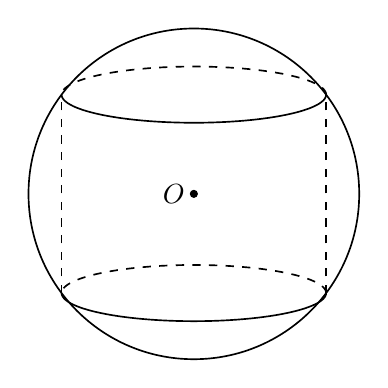
\begin{tikzpicture}[scale=1.05, >=stealth, semithick]
  % 球的大圆
  \draw (0,0) circle (2);

  % 圆柱上底：后半（上）虚线，前半（下）实线
  \draw[domain=0:180, samples=60, dashed] plot ({1.6*cos(\x)},{1.2+0.34*sin(\x)});
  \draw[domain=180:360, samples=60] plot ({1.6*cos(\x)},{1.2+0.34*sin(\x)});

  % 圆柱下底：后半（上）虚线，前半（下）实线
  \draw[domain=0:180, samples=60, dashed] plot ({1.6*cos(\x)},{-1.2+0.34*sin(\x)});
  \draw[domain=180:360, samples=60] plot ({1.6*cos(\x)},{-1.2+0.34*sin(\x)});

  % 圆柱的两条母线（原页为虚线）
  \draw[dashed] (-1.6,-1.2) -- (-1.6,1.2);
  \draw[dashed] (1.6,-1.2) -- (1.6,1.2);

  % 球心
  \fill (0,0) circle (1.4pt);
  \node[left, inner sep=3pt] at (0,0) {$O$};
\end{tikzpicture}
\end{center}
\nopagebreak[4]
\end{question}
\begin{question}
\gkti{16}函数 $f(x)$ 的定义域为 $A$，若 $x_1$，$x_2\in A$ 且 $f(x_1)=f(x_2)$ 时总有 $x_1=x_2$，则称 $f(x)$ 为单函数。例如，函数 $f(x)=2x+1$（$x\in\mathbf R$）是单函数。下列命题：

① 函数 $f(x)=x^2$（$x\in\mathbf R$）是单函数；

② 指数函数 $f(x)=2^x$（$x\in\mathbf R$）是单函数；

③ 若 $f(x)$ 为单函数，$x_1$，$x_2\in A$ 且 $x_1\neq x_2$，则 $f(x_1)\neq f(x_2)$；

④ 在定义域上具有单调性的函数一定是单函数。

其中的真命题是\gkblank{}。（写出所有真命题的编号）

\end{question}
\gkpart{三、解答题}

\begin{question}
\gkti{17}本着健康、低碳的生活理念，租自行车骑游的人越来越多。某自行车租车点的收费标准是每车每次租车时间不超过两小时免费，超过两小时的部分每小时收费 $2$ 元（不足 $1$ 小时的部分按 $1$ 小时计算）。有甲、乙两人相互独立来该租车点租车骑游（各租一车一次）。设甲、乙不超过两小时还车的概率分别为 $\dfrac14$、$\dfrac12$；两小时以上且不超过三小时还车的概率分别是 $\dfrac12$、$\dfrac14$；两人租车时间都不会超过四小时。

（1） 分别求出甲、乙在三小时以上且不超过四小时还车的概率；

（2） 求甲、乙两人所付的租车费用之和小于 $6$ 元的概率。

\end{question}
\begin{question}
\gkti{18}已知函数 $f(x)=\sin\left(x+\dfrac{7\pi}{4}\right)+\cos\left(x-\dfrac{3\pi}{4}\right)$，$x\in\mathbf R$。

（1） 求 $f(x)$ 的最小正周期和最小值；

（2） 已知 $\cos(\beta-\alpha)=\dfrac45$，$\cos(\beta+\alpha)=-\dfrac45$，$0<\alpha<\beta\leqslant\dfrac{\pi}{2}$，求证：$[f(\beta)]^2-2=0$。

\Needspace{0.4\textheight}
\end{question}
\begin{question}
\gkti{19}如图，在直三棱柱 $ABC-A_1B_1C_1$ 中，$\angle BAC=90^\circ$，$AB=AC=AA_1=1$。延长 $A_1C_1$ 至点 $P$，使 $C_1P=A_1C_1$，连接 $AP$ 交棱 $CC_1$ 于点 $D$。

（1） 求证：$PB_1\parallel$ 平面 $BDA_1$；

（2） 求二面角 $A-A_1D-B$ 的平面角的余弦值。
\nopagebreak[4]
\begin{center}% 2011 年四川卷文科第 19 题：直三棱柱 ABC-A1B1C1，D 在棱 CC1 上，P 在 A1C1 的延长线上，
%   且 C1P=A1C1，AD 的延长线过 D 交于 P。
% 来源 PDF：普通高考/2011/2011四川文.pdf，SHA-256 9df4a6b69bb06bfab2f7d7ee0e7fcc50ae547f226260996d7a060c31ad14e64a。
% 原页：第 2 页（A3 三栏）第 1 栏上部，书页码 704。
% 重绘依据：照原页——顶面 ABC 可见（AC 水平），B 在左、A 在上、C 在右上；BB1 为前面的竖棱（实线），
%   CC1 实线且 D 在其中点；A1 为被遮挡的顶点，A1B1、A1C1 为虚线，B1C1 实线；
%   实线：AB、AC、BC、BB1、CC1、BD、B1C1、DP、B1P、C1P；
%   虚线：AA1、A1B1、A1C1、BA1、A1D、AD。
%   P 在 A1C1 的延长线上（C1 之外），A1C1 段虚线、C1P 段实线，照原页；原页不画顶点圆点。
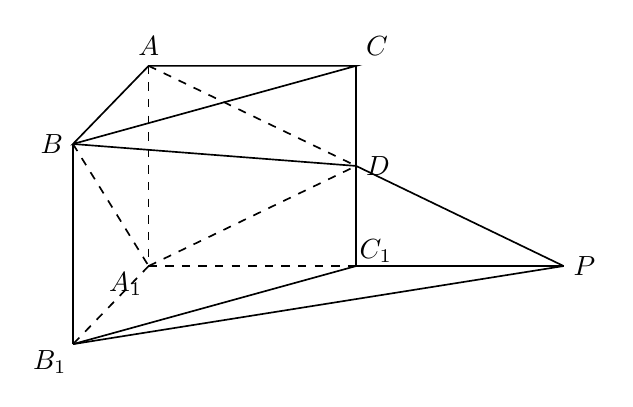
\begin{tikzpicture}[scale=0.62, >=stealth, semithick]
  \coordinate (A)  at (3.10,6.60);
  \coordinate (B)  at (1.55,5.00);
  \coordinate (C)  at (7.35,6.60);
  \coordinate (A1) at (3.10,2.50);
  \coordinate (B1) at (1.55,0.90);
  \coordinate (C1) at (7.35,2.50);
  \coordinate (D)  at (7.35,4.55);
  \coordinate (P)  at (11.60,2.50);

  % 可见的棱与辅助线（实线）
  \draw (A) -- (B) -- (C) -- cycle;
  \draw (B) -- (B1);
  \draw (C) -- (C1);
  \draw (B1) -- (C1);
  \draw (B) -- (D);
  \draw (D) -- (P);
  \draw (B1) -- (P);
  \draw (C1) -- (P);

  % 被遮挡的棱与辅助线（虚线）
  \draw[dashed] (A) -- (A1);
  \draw[dashed] (A1) -- (B1);
  \draw[dashed] (A1) -- (C1);
  \draw[dashed] (B) -- (A1);
  \draw[dashed] (A1) -- (D);
  \draw[dashed] (A) -- (D);

  \node at (A)  [above] {$A$};
  \node at (B)  [left] {$B$};
  \node at (C)  [above right] {$C$};
  \node at (A1) [below left, inner sep=2pt] {$A_1$};
  \node at (B1) [below left, inner sep=2pt] {$B_1$};
  \node at (C1) [above right, inner sep=1pt] {$C_1$};
  \node at (D)  [right] {$D$};
  \node at (P)  [right] {$P$};
\end{tikzpicture}
\end{center}
\nopagebreak[4]
\end{question}
\begin{question}
\gkti{20}已知 $\{a_n\}$ 是以 $a$ 为首项，$q$ 为公比的等比数列，$S_n$ 为它的前 $n$ 项和。

（1） 当 $S_1$，$S_3$，$S_4$ 成等差数列时，求 $q$ 的值；

（2） 当 $S_m$，$S_n$，$S_l$ 成等差数列时，求证：对任意自然数 $k$，$a_{m+k}$，$a_{n+k}$，$a_{l+k}$ 也成等差数列。

\Needspace{0.4\textheight}
\end{question}
\begin{question}
\gkti{21}过点 $C(0,1)$ 的椭圆 $\dfrac{x^2}{a^2}+\dfrac{y^2}{b^2}=1$（$a>b>0$）的离心率为 $\dfrac{\sqrt3}{2}$，椭圆与 $x$ 轴交于两点 $A(a,0)$，$B(-a,0)$，过点 $C$ 的直线 $l$ 与椭圆交于另一点 $D$，并与 $x$ 轴交于点 $P$，直线 $AC$ 与直线 $BD$ 交于点 $Q$。

（1） 当直线 $l$ 过椭圆右焦点时，求线段 $CD$ 的长；

（2） 当点 $P$ 异于点 $B$ 时，求证：$\overrightarrow{OP}\cdot\overrightarrow{OQ}$ 为定值。
\nopagebreak[4]
\begin{center}% 2011 年四川卷文科第 21 题：椭圆 x^2/4+y^2=1（即 a=2、b=1），顶点 A(2,0)、B(-2,0)，
%   C(0,1)，过 C 的直线 l 与椭圆交于另一点 D，交 x 轴于 P，直线 AC 与 BD 交于 Q。
% 来源 PDF：普通高考/2011/2011四川文.pdf，SHA-256 9df4a6b69bb06bfab2f7d7ee0e7fcc50ae547f226260996d7a060c31ad14e64a。
% 原页：第 2 页（A3 三栏）第 2 栏中部，书页码 704。
% 重绘依据：照原页——椭圆横长；B 为左顶点、A 为右顶点，C 在椭圆上、位于 y 轴正半轴；
%   l 自左上斜穿过 C，交 x 轴于 P（O 与 A 之间），再穿过椭圆上一点 D（第四象限）向右下延伸，
%   标号 l 在 D 的右下方；AC 自 A 过 C 向左上延长，BD 自 B 过 D 向右下延长，二者交于 Q（椭圆外右下方）。
%   取 l 的斜率 k=-1，此时 P(1,0)、D(8/5,-3/5)、Q(4,-1)，与原页各点相对位置一致；不按原页比例。
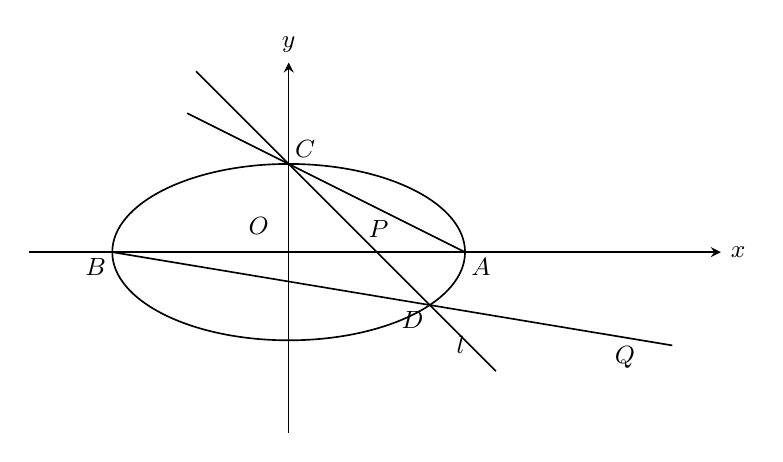
\begin{tikzpicture}[scale=1.12, >=stealth, semithick, font=\small]
  % 坐标轴
  \draw[->] (-2.95,0) -- (4.9,0) node[right] {$x$};
  \draw[->] (0,-2.05) -- (0,2.15) node[above] {$y$};

  % 椭圆
  \draw (0,0) ellipse (2 and 1);

  % 各点
  \coordinate (A) at (2,0);
  \coordinate (B) at (-2,0);
  \coordinate (C) at (0,1);
  \coordinate (D) at (1.6,-0.6);
  \coordinate (P) at (1,0);
  \coordinate (Q) at (4,-1);

  % 直线 l：自左上经 C、P、D 向右下
  \draw (-1.05,2.05) -- (2.35,-1.35);
  % 直线 AC 及其延长
  \draw (A) -- (-1.15,1.575);
  % 直线 BD 及其延长至 Q 并略过
  \draw (B) -- (4.35,-1.058);

  \node at (A) [below right, inner sep=2pt] {$A$};
  \node at (B) [below left, inner sep=2pt] {$B$};
  \node at (C) [above right, inner sep=2pt] {$C$};
  \node at (D) [below left, inner sep=2pt] {$D$};
  \node at (1.02,0.26) {$P$};
  \node at (Q) [below left, inner sep=2pt] {$Q$};
  \node at (-0.34,0.30) {$O$};
  \node at (1.95,-1.05) {$l$};
\end{tikzpicture}
\end{center}
\nopagebreak[4]
\end{question}
\begin{question}
\gkti{22}已知函数 $f(x)=\dfrac23x+\dfrac12$，$h(x)=\sqrt x$。

（1） 设函数 $F(x)=18f(x)-x^2[h(x)]^2$，求 $F(x)$ 的单调区间与极值；

（2） 设 $a\in\mathbf R$，解关于 $x$ 的方程 $\lg\left[\dfrac32f(x-1)-\dfrac34\right]=2\lg h(a-x)-2\lg h(4-x)$；

（3） 设 $n\in\mathbf N^*$，证明：$f(n)h(n)-[h(1)+h(2)+\cdots+h(n)]\geqslant\dfrac16$。

\end{question}